\chapter{Diskretes Äußeres Kalkül (DEC)}
\label{chapterDEC}

see \cite{Lee} \cite{FirstCourse}

\section{Diskrete Differentialformen}
  
  \begin{definition}
    Eine diskrete \( p \)-Form ist ein Homomorphismus vom Kettenkomplex \( C_{p}(K) \) nach \( \R \).
    Die Menge aller dieser Homomorphismen bezeichnen wir je nach Kontext mit \( C^{p}(K) \) (Menge der \( p \)-Koketten)
    oder \( \Omega^{p}_{d}(K) \) (Menge der diskrete \( p- \)(Differential-)Formen). 
    Das heißt
    \begin{align}
      \hom(C_{p}(K),\R) =: C^{p}(K) =: \Omega^{p}_{d}(K) \formpunkt
    \end{align}
    Desweiteren erfolgt die Addition punktweise, das heißt
    \begin{align}
      \left( \alpha + \beta \right)(c) &:= \alpha(c) + \beta(c)
    \end{align}
    für \( \alpha,\beta \in C^{p}(K) \) und \( c \in C_{p}(K) \).
  \end{definition}
  
  \begin{folgerung}
    \label{folgUnikKoketten}
    Da \( \R \) mit der Addition eine abelsche Gruppe ist, können wir uns wieder die Universalitätseigenschaft \eqref{diagFreieAbelscheGruppe} des Kettenkomplexes zunutze machen.
    Für eine \( p \)-Kette \( c = \sum_{\sigma\in K^{(p)}} a_{\sigma} \sigma \in C_{p}(K)\) und eine  \( p \)-Kokette \( \alpha\in C^{p}(K) \) gilt
    \begin{align}
      \alpha(c) &= \alpha\left(\sum_{\sigma\in K^{(p)}} a_{\sigma} \sigma\right) = \sum_{\sigma\in K^{(p)}} a_{\sigma} \alpha(\sigma) \formkomma
    \end{align}
    damit reicht es auch hier aus die \( p \)-Koketten nur auf den \( p \)-Simplizes zu definieren.
  \end{folgerung}

  Hätten wir die Menge der \( p \)-Ketten als \( \R \)-Vektoraum eingeführt, so hätte uns die Frage nach einem inneren Produkt zwischen den Ketten und den Koketten zur dualen Paarung
  geführt und damit auch, dass \( C^{p}(K) = \left( C_{p}(K) \right)^{*}\) der Dualraum von \( C_{p}(K) \) ist.
  Nun hält uns aber auch nichts davon ab, dies auch für die hier eingeführten Ketten analog zu machen.

  \begin{definition}
    \begin{align}
      \begin{aligned}
        \left\langle \bullet,\bullet \right\rangle : C^{p}(K) \times C_{p}(K)  &\rightarrow \R \\
                                                     \left( \alpha, c  \right) &\mapsto \left\langle \alpha, c \right\rangle := \alpha(c)
      \end{aligned}
    \end{align}
    heißt natürliche Paarung zwischen den \( p \)-Koketten (-Formen) und den \( p \)-Ketten.
  \end{definition}

  Die Verbindung zwschen diskreter Form und Differentialform ist die de-Rham-Abbildung.
  Dazu nehmen wir zunächst an, dass wir einen abstrakten Simplizialkomplex \( L \) vorliegen haben, das heißt, dass alle Simplizes auf der zugehörigen Mannigfaltigkeit \( M \) liegen.
  Das bringt erst einmal den Vorteil, dass Integration auf den Simplizes das gleiche Ergebinis auch auf der Mannigfaltigkeit liefert.

  \begin{definition}
    Die de-Rham-Abbildung bildet \( p \)-Differentialformen auf diskrete \( p \)-Formen (Koketten) ab. 
    Genauer
    \begin{align}
      \begin{aligned}
        \psi^{p}: \Omega^{p}(M) &\rightarrow C^{p}(L) = \Omega_{d}^{p}(L)\\
                       \alpha   &\mapsto \left( \sigma^{p} \mapsto \int_{\sigma^{p}} \alpha =: \psi^{p}(\alpha)(\sigma^{p}) =  \left\langle \psi^{p}(\alpha), \sigma^{p} \right\rangle\right)
                       \formkomma
      \end{aligned}
    \end{align}
    das heißt die diskrete \( p \)-Form \( \psi^{p}(\alpha) \in \Omega_{d}^{p}(L)  \) ist auf den \( p \)-Simplizes definiert, was wegen Folgerung \ref{folgUnikKoketten} vollkommen ausreicht.
  \end{definition}

  \begin{folgerung}
    Zum einen ist \( \psi \) linear, da das Integral ein lineares Funktional ist.
    Zum anderen ist die de-Rham-Abbildung surjektiv.
    Das hat den Vorteil, dass sich jedes \( \alpha_{d}\in\Omega_{d}^{p}(L) \) auch als \( \psi(\alpha) = \alpha_{d} \) schreiben lässt, da
    immer solch ein geeignetes \( \alpha\in\Omega^{p}(M) \) existiert.
    \begin{proof}
      Da es ausreicht die Aussage für eine Basis von \( \Omega_{d}^{p}(L) \) zu zeigen, nehmen wir einfach die duale Basis 
      \begin{align}
        \left(L^{(p)}\right)^{*} 
            &:= \left\{\sigma_{i}^{*} \in \Omega_{d}^{p}(L) \middle| \sigma_{i}^{*}(\sigma_{j}) = \delta_{ij}
                                ,\, i,j=1,\ldots,m \right\} \formkomma
      \end{align}
      wobei \( m \) die Anzahl der \( p \)-Simplizes in \( L^{(p)} \) ist und \( \delta_{ij} \) das Kronecker-Delta.
      Nun brauchen wir für \(i=1,\ldots,m \) nur noch geeignete \( \alpha_{i}\in\Omega^{p}(M) \) finden, so dass
      \begin{align}
        \label{eq}
        \int_{\sigma_{j}} \alpha_{i} &= \delta_{ij}
      \end{align}
      gilt. Es sei dazu eine auf \( \sigma_{i}\subset M \) lokale Basis \( \left( x^{1},\ldots,x^{p} \right) \) gegeben, dann definieren
      wir eine \( p \)-Form auf dem Polytop von \( L^{(p)} \)
      \begin{align}
        \alpha_{i} &:= \frac{1}{|\sigma_{i}|} \chi_{\sigma_{i}} dx^{1}\wedge\ldots\wedge dx^{p} \in \Omega^{p}(|L^{(p)}|) \formkomma
      \end{align}
      wobei \( \chi \) die Indikatorfunktion ist.
      Mit der Inklusionsabbildung \( \iota: |L^{(p)}| \hookrightarrow M\) erfüllt gerade der Pullback (s.u.
      \eqref{eqPullbackEntlangInklusion})
      \( \iota^{*}\alpha_{i}\in\Omega^{p}(M) \) die Anforderung \eqref{eq} 
      und damit auch \( \psi(\iota^{*}\alpha_{i}) = \sigma^{*}_{i} \).
    \end{proof}
  \end{folgerung}
  \todo{whitney abbildung noch ansprechen? Das heißt Interpolation im allgemeinen oder nur speziell?}

  \begin{bemerkung}
    Nun haben wir bei der Definition der de-Rham-Abbildung vorrausgesetzt, dass ein abstrakter Simplizialkomplex vorliegt.
    Das entspricht aber nur für flache Mannigfaltigkeiten unseren Anfoderungen.
    Im Allgemeinen ist die gegebene Triangulation nur eine lineare Approximation der Mannigfaltigkeit und damit auch des zugehörigen abstrakten Simplizialkomplexes.
    Das bedeutet auch, dass für \( p \ge 1 \) die Differentialformen von \( M \) in einem anderen Raum "`leben"' als die Differentialformen des Polytopes \( |K| \).
    Rein formal ließe sich die Situation entschärfen, in dem wir die Simplizes von \( K \) auf die Mannigfaltigkeit projizieren (vgl. \eqref{diagSingulaerAbstrakt}), also es wird
    \( \left\langle \psi^{p}(\alpha), \pi(\sigma^{p}) \right\rangle = \left( \psi^{p}(\alpha) \circ \pi \right)(\sigma^{p}) \) gerechnet für ein \( \sigma^{p}\in K \).
    Nur ist in vielen praktischen Aufgaben weder die Projektion noch die Mannigfaltigkeit exakt bekannt, so bleibt also nur die approximative Auswertung des Integrals.
    Wir werden deshalb auch einfach  \( \left\langle \alpha_{d}, \sigma^{p} \right\rangle \) statt \( \left\langle \alpha_{d}, \pi(\sigma^{p}) \right\rangle \) schreiben.
    Für die numerische Analysis ist das eine schwierige Situation, da vor der eigentlichen Diskretisierung (Diskretisierungsfehler) noch eine Approximation (geometrischer Fehler) auf einen stückweise
    flachen Raum gemacht wird.

    Für \( 0 \)-Formen (identisch zu Skalarfeldern) ergibt sich dieser geometrische Fehler nicht, da nach Vorraussetzung die Ecken des Simplizialkomplexes auf der Mannigfaltigkeit liegen.
    Hier ist die Diskretisierung genauso wie wir das aus anderen Verfahren, wie die Finite-Differenzen-Methode, gewöhnt sind, da das "`Punktintegral"' nichts weiter als die Auswertung an
    eben diesem Punkt ist.
    Das heißt, liegt ein Skalarfeld \( u:M\rightarrow\R \) vor, so ist das diskrete Skalarfeld \( u_{d}:K^{(0)} \rightarrow \R \) an den Ecken definiert.
    \begin{align}
      u(v_{i}) &=  \psi(u)(v_{i}) = \left\langle \psi(u), v_{i} \right\rangle= u_{d}(v_{i}) =: u_{i} 
    \end{align}
    für alle \( v_{i} \in K^{(0)} \).
    Die Interpolation zurück zur Mannigfaltigkeit kann dann mittels linearer Ansatzfunktionen erfolgen, die sich auf den Volumenenelementen \( \sigma^{n} \) in gewohnter
    Weise definieren, das heißt 1 auf einer ausgezeichneten Ecke und 0 auf den übrigen Ecken.
    In dieser Arbeit werden wir uns auf die Auswertung von \( 0 \)-Formen beschränken, das reicht aus um skalarwertige oder vektorisierte skalarwertige Differentialgleichungen höherer
    Ordnung zu diskretisieren.

    Dennoch sei hier auf die Auswertung von \( 1 \)-Formen (Pfaffsche Formen) eingegangen, 
    denn sie werden zum einen für spätere numerischen Betrachtungen und zum anderen für die Behandlung von (Tangential-)Vektorproblemen
    noch interessant werden, denn mittels \( \flat \) beziehungsweise \( \sharp \) ist ein Isomorphismus zwischen Vektorfeldern und \( 1 \)-Formen gegeben.
    Betrachten wir hierzu eine \( 1 \)-Form \( \alpha\in\Omega^{1}(M) \) und die zugehörige diskrete Form \( \alpha_{d} = \psi(\alpha)\in\Omega^{1}_{d}(M) \).
    Wie sind diese beiden Formen zu vergleichen? 
    Beide geben haben zwar Antworten in \( \R \) aber die Differentialform nimmt einen Tangentialvektor und die diskrete Form eine Kante als Eingabe. 
    Dazu sei eine Kante \( \sigma^{1}_{\eps} \in K\) der Länge \( 2\eps \) gegeben und deren abstrakte Kante \( s_{\eps}\in L \), die auf der Mannigfaltigkeit liegt, 
    siehe Abbildung \ref{figDiskrete1Form}.
    \( s_{\eps}: (-\eps,\eps)\rightarrow M \) sei in Parameterform gegeben und zwar so, dass \( s_{\eps}(0)=x_{0}\in M \), \( \dot{s}_{\eps}(0) = v \in T_{x_{0}}M \) 
    und \( x_{0}\in M \subset \R^{N} \) so gewählt, dass \( v \) parallel zur Kante \( \sigma^{1}_{\eps} \) ist (Existenz folgt aus dem Mittelwertsatz der Differentialrechnung).
    Ohne Einschränkung der Allgemeinheit sei \( v \) der tangential Einheitsvektor in der umgebenen \( \xi \)-\( \eta \)-Ebene.
    Die Auswertung der diskreten Form an der Kante \( \sigma^{1}_{\eps} \) ergibt
    \begin{align}
        \alpha_{d}(\sigma_{\eps}^{1}) &= \langle \psi(\alpha) , s_{\eps} \rangle = \int_{s_{\eps}}\alpha = \int_{-\eps}^{\eps} (\alpha \circ \dot{s}_{\eps})(t) dt\\
                                 &\approx 2\eps \alpha(v) \formpunkt
    \end{align}
    Mit \( |\sigma^{1}_{\eps}| = 2\eps \) folgt 
    \begin{align}
    \label{eqApprox1Form}
      \frac{1}{|\sigma^{1}_{\eps}|} \alpha_{d}(\sigma_{\eps}^{1}) = \text{"`}\alpha_{d}(v)\text{"'} \approx \alpha(v)\formpunkt
    \end{align}
    \( \alpha_{d}(v) \) ist in Anführungszeichen gesetzt, da die diskreten Formen diese schreibweise nicht hergeben (\( v \cong \nicefrac{\sigma^{1}_{\eps}}{|\sigma^{1}_{\eps}|} \notin K \)), 
    aber wir wollen hier auf unnötigen Formalismus verzichten und uns ist
    klar was damit gemeint ist.
    Das Integral wurde an \( t=0 \) aproximiert, also mit der Mittelpunktsregel.
    Daher können wir abschätzen (siehe \cite{einfNum}, Kapitel 7)
    \todo{bei langeweile s mal explizit in lok.koords aufstellen um den Fehler besser abzuschätzen}
    \begin{align}
    \begin{aligned}
      \left| \text{"`}\alpha_{d}(v)\text{"'} - \alpha(v) \right|
              &\le \frac{(2\eps)^{3}}{24} \frac{1}{2\eps} \max_{\tau\in(-\eps,\eps)} \left|\frac{d^{2}(\alpha \circ\dot{s}_{\eps})}{dt^{2}}(\tau) \right| \\
              &= \frac{\eps^{2}}{6} \max_{\tau\in(-\eps,\eps)} \left|\frac{d^{2}(\alpha \circ \dot{s}_{\eps})}{dt^{2}}(\tau) \right| \formpunkt
    \end{aligned}
    \end{align}
    \begin{figure}
      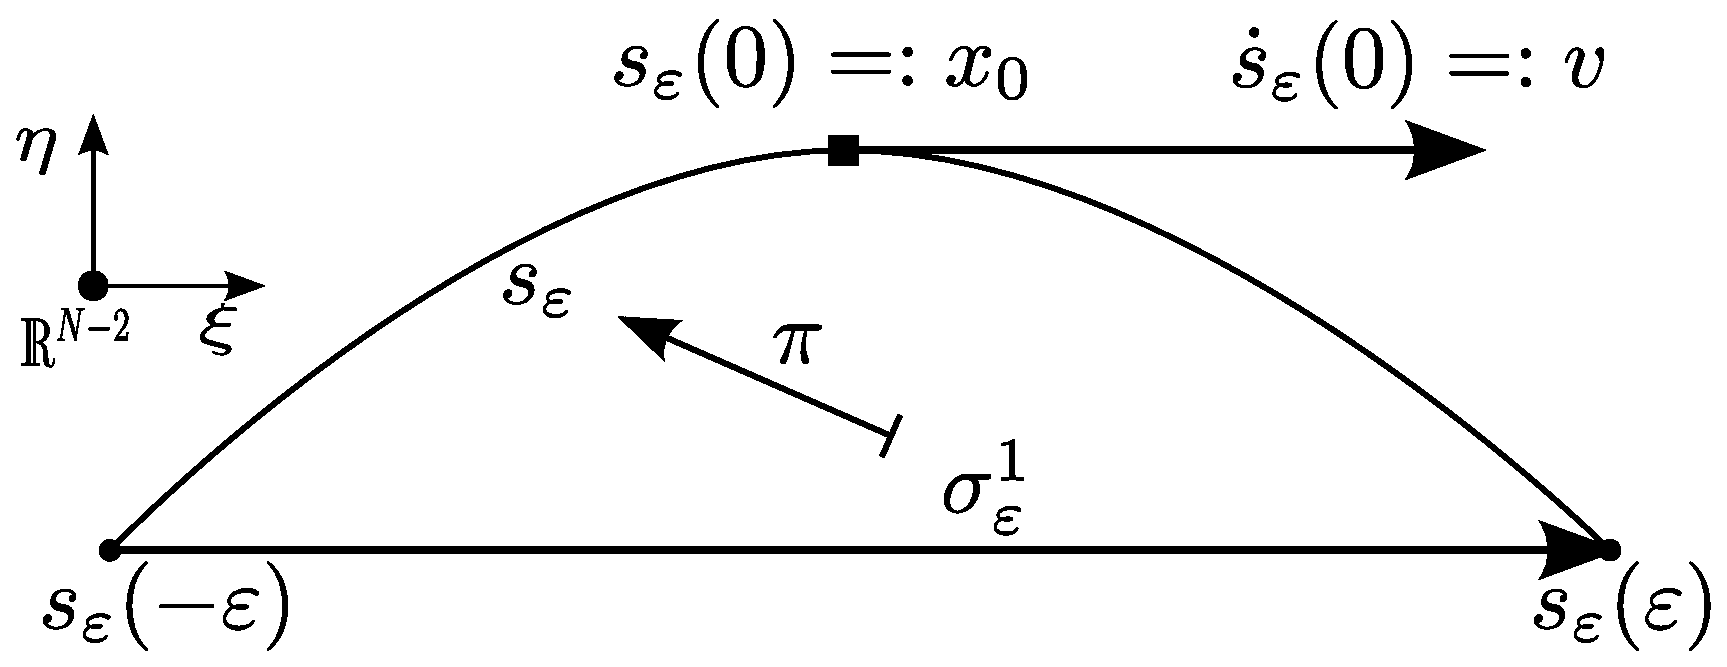
\includegraphics[width=\textwidth]{bilder/EpsilonKette.eps}
      \caption[Approximation einer 1-Form]{Das umliegende Koordinatensystem ist so gedreht, dass die Kante \( \sigma_{\eps}^{1} \) und die zugehörige abstrakte Kante \( s_{\eps} \)
                                           in der \( \xi \)-\( \eta \)-Ebene liegen. Die übrigen \( (N-2) \) Dimensionen zeigen aus der Bildebene heraus.
                                           \( \pi \) klebt die Kante auf die Mannigfaltigkeit, d.h. \( \pi(\sigma_{\eps}^{1}) = s_{\eps} \)}
      \label{figDiskrete1Form}
    \end{figure}
    Das soll nicht heißen, dass die \( 1 \)-Form \( \alpha\in\Omega^{1}(M) \) mit mindestens Ordnung 2 approximiert wird, denn im hinteren Faktor steckt noch immer die Größe \( \eps \)
    und \( s_{\eps} \) hängt zudem stark von der Geometrie der Mannigfaltigkeit ab.
    Wenn allerdings die Mannigfaltigkeit über der Kante \( \sigma^{1}_{\eps} \) flach wäre, dann ergibt sich \( s_{\eps}(t)=t v  \) für
    \( x_{0} = c(\sigma^{1}_{\eps}) = \vec{0} \) (alle \( x_{0} \) erfüllen hier \( \dot{s}_{\eps}(x_{0}) \| \sigma_{\eps}^{1} \)).
    Daraus folgt, dass
    \begin{align}
      \left| \text{"`}\alpha_{d}(v)\text{"'} - \alpha(v) \right| 
            &\le \frac{\eps^{2}}{6} \max_{\tau\in(-\eps,\eps)} \left|\frac{\partial^{2}\alpha_{\xi}}{\partial\xi^{2}}(\tau v) \right| \formkomma
    \end{align}
    wobei \( \alpha_{\xi} = \alpha(\frac{\partial}{\partial\xi})=\alpha(v) \) die entsprechende (kovariante) Koordinatenfunktion von \( \alpha \) ist.
    Somit hätten wir Konsistenz der Ordnung 2 für den flachen Fall.
    In zukünftigen Arbeiten müsste also "`nur"' noch geklärt werden mit welcher Ordnung eine "`flache"' 1-Form aus \( \Omega^{1}(\sigma^{1}_{\eps}) \) eine
    "`gekrümmte"' 1-Form aus \( \Omega^{1}(\pi(\sigma^{1}_{\eps}))\subset\Omega^{1}(M) \) approximiert.
    
    Dagegen lässt sich für exakte \( 1 \)-Formen tatsächlich eine Ordnung von 2 direkt abschätzen.
    Sei eine exakte Form \( \alpha\in\Omega^{1}(M) \) gegeben, das heißt es existiert ein \( f\in\Omega^{0}(M) \), sodass \( \alpha= \exd f \) gilt.
    Mit dem Stokes Theorem (\cite{Marsden}, Kapitel 7.2) erhalten wir
    \begin{align}
    \label{eqExakt1FormPart1}
      \frac{1}{|\sigma^{1}_{\eps}|} \alpha_{d}(\sigma_{\eps}^{1}) &= \frac{1}{|\sigma^{1}_{\eps}|}\int_{s_{\eps}}\alpha 
                                                                   = \frac{1}{2\eps}\int_{\partial s_{\eps}} f
                                                                   = \frac{(f\circ s_{\eps})(\eps) - (f\circ s_{\eps})(-\eps)}{2\eps} \formpunkt
    \end{align}
    Wenn wir \( \left( x^{1},\ldots,x^{n} \right) \) als lokale Koordinaten der \( n \)-Mannigfaltigkeit am Punkt \( x_{0} \) wählen, 
    so dass \( x^{1} \) gerade die Standartkoordinate entlang der abstrakten Kante \( s_{\eps} \) ist mit \( v=\dot{s}_{\eps}(0) \) als tangentialer Einheitsvektor,
    also für die dualen Basisvektoren gilt 
    \begin{align}
      dx^{i}(v) &= \begin{cases}
                      1 & \text{falls } i=1 \\
                      0 & \text{sonst}
                  \end{cases} \formkomma
    \end{align}
    dann ergibt sich am Punkt \( x_{0}= s_{\eps}(0) \)
    \begin{align}
    \label{eqExakt1FormPart2}
      \begin{aligned}
        \alpha(v) &= \left( \exd f \right)(v) = \sum_{i=1}^{n}\frac{\partial f}{\partial x^{i}} dx^{i}(v)
                   = \nabla_{M}f \cdot v
                   = \nabla_{M}f \cdot \dot{s}_{\eps}
                   = \frac{d (f\circ s_{\eps})}{dt}(0) \formpunkt
      \end{aligned}
    \end{align}
    Da \eqref{eqExakt1FormPart1} nichts weiter als der Zentrale Differenzenquotient von \eqref{eqExakt1FormPart2} ist gilt
    \begin{align}
      \left| \text{"`}\alpha_{d}(v)\text{"'} - \alpha(v) \right| = \mathcal{O}(\eps^{2}) \formpunkt
    \end{align}

    Wir könnten nun auch ähnliche Betrachtungen für Differentialformen höheren Grades anstellen, jedoch werden wir uns im praktischen Teil nur auf zweidimensionale Oberflächen beschränken.
    Damit bleiben nur noch die \( 2 \)-Formen übrig und die unterscheiden sich wegen dem Hodge-Stern-Isomorphismus nur um einen geometrischen Faktor (und Syntax) von den \( 0 \)-Formen.
    Das heißt, wenn eine Riemannsche Mannigfaltigkeit vorliegt mit metrischen Tensor \( g \), dann gilt für alle \( 2 \)-Formen \( f \, dx^{1}\wedge dx^{2} \in \Omega^{2}(M)\), dass
    \begin{align}
      \label{eqHodgeIso2Form}
      * \left( f \, dx^{1}\wedge dx^{2} \right) = \frac{f}{\sqrt{|\det(g)|}} \in \Omega^{0}(M) \formpunkt
    \end{align}
  \end{bemerkung}




  
  

\section{Äußere Ableitung}
  
  Wenn wir uns den de-Rham-Komplex anschauen, also die für eine \( n \)-Mannigfaltigkeit eindeutig festgelegte Sequenz
    \begin{align}
      \begin{xy}
        \xymatrix{
          0 \ar[r] & 
          \Omega^{0}(M) \ar[r]^{\exd^{0}} &
          \Omega^{1}(M) \ar[r]^{\exd^{1}} &
          \ldots \ar[r]^{\exd^{n-1}} &
          \Omega^{n}(M) \ar[r] &
          0 \\
        }
      \end{xy}
    \end{align}
  mit den äußeren Ableitungen (Cartansche Ableitungen) \( \exd^{i} \), dann kommt uns das irgendwie bekannt vor.
  Dieser Kokettenkomplex mit der Komplexeigenschaft \( \exd\circ\exd \equiv 0 \) (auf die Indizierung kann wieder verzichtet werden) ähnelt
  doch sehr dem simplizialen Kettenkomplex aus Folgerung \ref{folgSimplizialerKettenkomplex} mit dem Unterschied, dass die lineare
  Abbildung \( \exd \) "`in eine andere Richtung zeigt"' als der lineare Randoperator \( \partial \).
  Und tatsächlich gibt es eine Verbindung zwischen diesen beiden Komplexen.
  Es ist der Satz von Stokes 
  (\cite{Marsden}(Kap. 7.2), \cite{jaenich}(Kap. 9))
  , den wir im vorherigen Abschnitt auch schon benutzt hatten.
  Wir wollen ihn hier nochmal kurz niederschreiben.

  \begin{satz}[Satz von Stokes]
    Es sei \( U \) eine orientierte \( p \)-dimensionale berandete Mannigfaltigkeit und \( \alpha\in\Omega^{p-1}(U) \) eine \( (p-1)\)-Form
    mit kompakten Träger.
    Dann gilt
    \begin{align}
      \int_{U} \exd\alpha &= \int_{\partial U} \alpha \formpunkt
    \end{align}
    Dabei ist formal etwas Vorsicht geboten, denn \( \alpha \) ist eine Differentialform auf \( U \) und nicht auf dessen Rand.
    Deshalb müssen wir uns die Inklusionsabbildung \( \iota:\partial U \hookrightarrow U \) dazu denken und nutzen die entlang dieser Abbildung
    zurückgezogene Differentialform \( \iota^{*}\alpha\in\Omega^{p-1}(\partial U) \) (Pullback).
    Das heißt
    \begin{align}
      \int_{\partial U} \alpha &:= \int_{\partial U} \iota^{*}\alpha \formpunkt
    \end{align}
    Diese Kurzschreibweise ist berechtigt, denn es gilt für alle \( x\in\partial U \), dass
    \begin{align}
    \label{eqPullbackEntlangInklusion}
      (\iota^{*}\alpha)_{x}(v_{1},v_{2},\ldots,v_{p-1}) = \alpha_{x}(v_{1},v_{2},\ldots,v_{p-1}) \formpunkt
    \end{align}
    und da beide Formen auf dem Rand lokal die gleichen Antworten in \( \R \) liefern, spielt das auch für die Integralauswertung keine Rolle.
  \end{satz}

  \begin{definition}
    \label{defAeussereAbleitung}
    Für eine Mannigfalligkeit \( M \) und einem Primärgitter \( K \) heißt 
    \begin{align}
      \label{eqAeussereAbleitung}
      \begin{aligned}
        \exd : \Omega^{p}_{d}(K) &\rightarrow \Omega^{p+1}_{d}(K) \\
               \psi(\alpha) &\mapsto \exd\psi(\alpha):=\psi(\exd \alpha)
      \end{aligned}
    \end{align}
    diskrete äußere Ableitung.
  \end{definition}
    

  \begin{folgerung}
    Die diskrete äußere Ableitung lässt sich mit Hilfe des Satzes von Stokes und den Randoperator berechnen.
    Es sei \( \alpha_{d}=\psi(\alpha)\in\Omega_{d}^{p}(K) \) eine diskrete \( p \)-Form und \( \sigma\in K^{(p+1)} \) ein \( (p+1) \)-Simplex, dann gilt
    \begin{align}
      \left\langle \exd\alpha_{d} , \sigma \right\rangle &= \int_{\pi_{\sigma}(\sigma)} \exd\alpha 
                                                          = \int_{\partial\pi_{\sigma}(\sigma)} \alpha
                                                          = \int_{\pi_{\partial\sigma}(\partial\sigma)} \alpha
                                                          = \left\langle \alpha_{d} , \partial\sigma \right\rangle
    \end{align}
    mit \( \pi_{\sigma}|_{\partial\sigma} = \pi_{\partial\sigma} \).
    Deshalb bezeichnen wir \eqref{eqAeussereAbleitung} auch als Korandoperator.
    Des Weiteren ist somit Definition \ref{defAeussereAbleitung} representantenunabhängig (Wohldefiniertheit),
    denn wenn \( \alpha_{1},\alpha_{2} \in \Omega^{p}(M) \) mit \( \psi(\alpha_{1}) = \psi(\alpha_{2}) \), 
    dann gilt für alle \( \sigma\in K^{(p+1)} \), dass
    \begin{align}
      \left\langle \exd\psi(\alpha_{1}), \sigma \right\rangle &= \left\langle \psi(\alpha_{1}), \partial\sigma \right\rangle
                                                               = \left\langle \psi(\alpha_{2}), \partial\sigma \right\rangle
                                                               = \left\langle \exd\psi(\alpha_{2}), \sigma \right\rangle
    \end{align}
  \end{folgerung}
  
  \begin{bemerkung}
    Betrachten wir nun im speziellen wieder ein zweidimensionales Primärgitter \( K \) beziehungsweise dessen Dualgitter \( \csd K \), 
    falls \( K \) wohlzentriert ist.
    Da das Dualgitter wiederum auch ein Primärgitter ist, gelten obige Definitionen dieses Abschnittes auch auf diesem. 
    \todo{verweis auf Koketten C(*K) }
    Somit ergeben sich folgende Berechnungsformeln.\\
    \begin{tabular}{|c|c|} \hline
      Darstellung & Formel \\\hline
      \begin{minipage}[c]{0.29\textwidth}
        \centering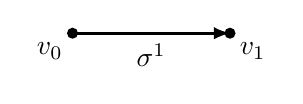
\begin{tikzpicture}[>=latex]
  % Coords
  \coordinate (V0) at (0,0);
  \coordinate (V1) at (2,0);
  \draw[line width=1pt, ->]
    (V0) -- node[below] {\( \sigma^{1} \)} (V1);
  % Points
  \fill (V0) node[below left] {\( v_{0} \)} circle (2pt);
  \fill (V1) node[below right] {\( v_{1} \)} circle (2pt);
\end{tikzpicture}


      \end{minipage} &
      \begin{minipage}[c]{0.69\textwidth}
        Für \( f\in\Omega_{d}^{0}(K) \) und \( \sigma^{1}=\left[ v_{0}, v_{1} \right]\in K \) gilt
        {\begin{align}
          \label{eqAbleitungKante}
          \left\langle \exd f , \sigma^{1} \right\rangle &= f(v_{1}) - f(v_{0}) \formpunkt
        \end{align}}
      \end{minipage} \\\hline
      \begin{minipage}[c]{0.29\textwidth}
        \centering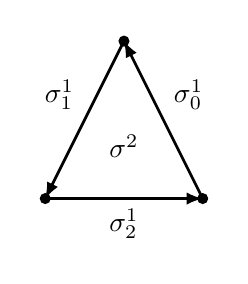
\begin{tikzpicture}[>=latex]
  % Coords
  \coordinate (V0) at (0,0);
  \coordinate (V1) at (2,0);
  \coordinate (V2) at (1,2);
  % Arrows\tilde{\sigma}
  \draw[line width=1pt, ->]
    (V0) -- node[below] {\( \sigma^{1}_{2} \)} (V1);
  \draw[line width=1pt, ->]
    (V1) -- node[above right] {\( \sigma^{1}_{0} \)} (V2);
  \draw[line width=1pt, ->]
    (V2) -- node[above left] {\(\sigma^{1}_{1}  \)} (V0);
  % Points
  \fill (V0) circle (2pt);
  \fill (V1) circle (2pt);
  \fill (V2) circle (2pt);
  % center
  \coordinate (C) at (1,0.666);
  \node at (C) {\( \sigma^{2} \)};

  \useasboundingbox ([shift={(1mm,1mm)}]current bounding box.north east) rectangle ([shift={(-1mm,-1mm)}]current bounding box.south west);
\end{tikzpicture}


      \end{minipage} &
      \begin{minipage}[c]{0.69\textwidth}
      Für \( \alpha\in\Omega_{d}^{1}(K) \) und \( \sigma^{2},\sigma^{1}_{0},\sigma^{1}_{1},\sigma^{1}_{2} \in K \) 
      mit \( \partial\sigma^{2} = \sum_{i=0}^{2} \sigma^{1}_{i} \) gilt
        {\begin{align}
          \left\langle \exd \alpha , \sigma^{2} \right\rangle &= \sum_{i=0}^{2} \left\langle \alpha, \sigma_{i}^{1}\right\rangle
        \end{align}}
      \end{minipage} \\\hline
      \begin{minipage}[c]{0.29\textwidth}
        \centering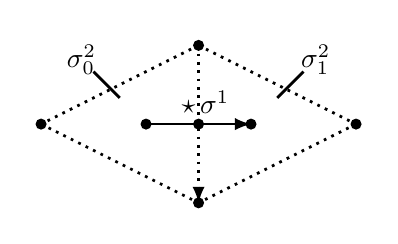
\begin{tikzpicture}[>=latex]
  % Coords
  \coordinate (V0) at (2,0);
  \coordinate (V1) at (2,2);
  \coordinate (V2) at (0,1);
  \coordinate (V3) at (4,1);
  % Arrows\tilde{\sigma}
  \draw[line width=1pt, ->, style=dotted]
    (V1) -- (V0);
  \draw[line width=1pt, style=dotted]
    (V1) --  (V2);
  \draw[line width=1pt, style=dotted]
    (V2) -- (V0);
  \draw[line width=1pt, style=dotted]
    (V1) --  (V3);
  \draw[line width=1pt, style=dotted]
    (V3) -- (V0);
  % Points
  \fill (V0) circle (2pt);
  \fill (V1) circle (2pt);
  \fill (V2) circle (2pt);
  \fill (V3) circle (2pt);
  %circumcenter
  \coordinate (CC0) at (1.333,1);
  \coordinate (CC1) at (2.666,1);
  \coordinate (CCC) at (2,1);
  \fill (CC0) circle (2pt);
  \fill (CC1) circle (2pt);
  \fill (CCC) circle (2pt);
  \draw[line width=1pt, ->]
    (CC0) -- node[above] {\( \,\,\,\star\,\sigma^{1} \)} (CC1);
  % nodes
  \draw[line width=1pt]
    (0.666,1.666) -- node[above left] {\( \sigma^{2}_{0} \)} (1,1.333);
  \draw[line width=1pt]
    (3.333,1.666) -- node[above right] {\( \sigma^{2}_{1} \)} (3,1.333);
	
\useasboundingbox ([shift={(1mm,1mm)}]current bounding box.north east) rectangle ([shift={(-1mm,-1mm)}]current bounding box.south west);
\end{tikzpicture}


      \end{minipage} &
      \begin{minipage}[c]{0.69\textwidth}
        Für \( f\in\Omega_{d}^{0}(\csd K) \), \( \sigma^{2}_{0}, \sigma^{2}_{1} \in K \) und 
        \( \star\sigma^{1} \in \star K \) gilt
        {\begin{align}
          \left\langle \exd f , \star\sigma^{1} \right\rangle &= f(c(\sigma^{2}_{1})) - f(c(\sigma^{2}_{0})) \formpunkt
        \end{align}}
      \end{minipage} \\\hline
      \begin{minipage}[c]{0.30\textwidth}
        \centering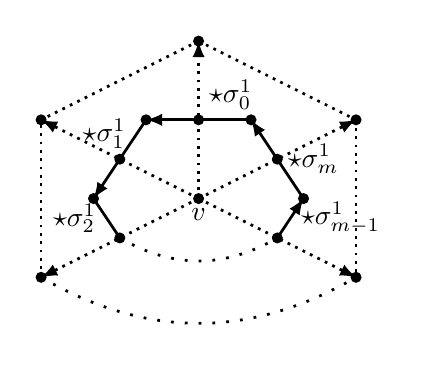
\begin{tikzpicture}[>=latex]
  % Coords
  \coordinate (V0) at (2,0);
  \coordinate (V1) at (2,2);
  \coordinate (V2) at (0,1);
  \coordinate (V3) at (4,1);
  \coordinate (V4) at (4,-1);
  \coordinate (V5) at (0,-1);
  % Arrows\tilde{\sigma}
  \draw[line width=1pt, ->, style=dotted]
    (V0) -- (V1);
  \draw[line width=1pt, style=dotted]
    (V1) --  (V2);
  \draw[line width=1pt, ->, style=dotted]
    (V0) -- (V2);
  \draw[line width=1pt, style=dotted]
    (V1) --  (V3);
  \draw[line width=1pt, ->, style=dotted]
    (V0) -- (V3);
   \draw[line width=1pt, ->, style=dotted]
    (V0) -- (V4);
  \draw[line width=1pt, ->, style=dotted]
    (V0) -- (V5);
  \draw[line width=1pt, style=dotted]
    (V5) --  (V2);
  \draw[line width=1pt, style=dotted]
    (V3) --  (V4);
  % Points
  \fill (V0) node[below] {\(v\)} circle (2pt);
  \fill (V1) circle (2pt);
  \fill (V2) circle (2pt);
  \fill (V3) circle (2pt);
  \fill (V4) circle (2pt);
  \fill (V5) circle (2pt);
  \draw[line width=1pt, style=loosely dotted]
     (V5) to[bend right] (V4);
  %circumcenter
  \coordinate (CC1) at (1.333,1);
  \coordinate (CC0) at (2.666,1);
  \coordinate (CC2) at (0.666,0);
  \coordinate (CCm) at (3.333,0);
  \coordinate (CCC0) at (2,1);
  \coordinate (CCC1) at (1,0.5);
  \coordinate (CCC2) at (3,0.5);
  \coordinate (CCC3) at (1,-0.5);
  \coordinate (CCC4) at (3,-0.5);
  \fill (CC0) circle (2pt);
  \fill (CC1) circle (2pt);
  \fill (CC2) circle (2pt);
  \fill (CCm) circle (2pt);
  \fill (CCC0) circle (2pt);
  \fill (CCC1) circle (2pt);
  \fill (CCC2) circle (2pt);
  \fill (CCC3) circle (2pt);
  \fill (CCC4) circle (2pt);
  \draw[line width=1pt, ->] (CC0) -- node[above right] {\(\star\sigma_0^1\)} (CC1);
  \draw[line width=1pt, ->] (CC1) -- node[above left] {\(\star\sigma_1^1\hspace{-6pt}\)}(CC2);
  \draw[line width=1pt, ->] (CCm) -- node[right] {\(\star\sigma_m^1\)} (CC0);
  \draw[line width=1pt,] (CC2) -- node[left] {\(\star\sigma_2^1\)} (CCC3);
  \draw[line width=1pt,->] (CCC4) -- node[right] {\(\star\sigma_{m-1}^1\)} (CCm);
  \draw[line width=1pt, style=loosely dotted]
     (CCC3) to[bend right] (CCC4);

	
\useasboundingbox ([shift={(1mm,1mm)}]current bounding box.north east) rectangle ([shift={(-1mm,-1mm)}]current bounding box.south west);
\end{tikzpicture}


      \end{minipage} &
      \begin{minipage}[c]{0.68\textwidth}
        Für \( \alpha\in\Omega_{d}^{1}(\csd K) \) und \( \star v, \star\sigma_{i}^{1} \in \star K \) mit
        \( \partial(\star v) = \sum_{i=0}^{m} \star\sigma_{i}^{1} \) und \( \sigma_{i}^{1} \succ v  \) gilt
        {\begin{align}
          \left\langle \exd \alpha , \star v \right\rangle &=  \sum_{i=0}^{m} \left\langle \alpha, \star\sigma_{i}^{1}\right\rangle
          \formkomma
        \end{align}}
        wobei \( (m+1) \) die Anzahl der Kanten ist, die \( v \) als Ecke haben.
      \end{minipage} \\\hline
    \end{tabular}
    Die Orientierungen der Kanten wurden dabei so gewählt, dass möglichst wenig Vorzeichenwechsel entstehen.
  \end{bemerkung}

  Alleine mit der äußeren Ableitung ließe sich auf einer \( 2 \)-Mannigfaltigkeit schon einiges Rechnen.
  Sie definiert uns nämlich den Gradienten eines (glatten) Skalarfeldes 
  \begin{align}
    \begin{aligned}
      \nabla: C^{\infty}(M) &\rightarrow \mathcal{V}^{\infty}(M) \\
                            f  &\mapsto \left( \exd f \right)^{\sharp}
                                        = \left[ g^{1} \frac{\partial f}{\partial x^{1}}, g^{2} \frac{\partial f}{\partial x^{2}} \right]^{T}
    \end{aligned}
  \end{align}
  und die Rotation eines (glatten) (Tangential-)Vektorfeldes
  \begin{align}
    \begin{aligned}
      \text{rot}: \mathcal{V}^{\infty}(M) &\rightarrow C^{\infty}(M) \\
                \vec{v} = \left[ v^{1}, v^{2} \right]^{T} &\mapsto * \exd (\vec{v})^{\flat}
                                                           = \frac{1}{\sqrt{|\det g|}}\left( \frac{\partial g_{2}v^{2}}{\partial x^{1}} -  \frac{\partial g_{1}v^{1}}{\partial x^{2}}\right)
    \end{aligned}
  \end{align}
  für ein lokales orthogonales\footnote{o.E.d.A, da die riemannsche Metrik \( g  \) lokal positiv definit und symetrisch ist, also auch diagonalisierbar} 
  Koordinatensystem \( (x^{1}, x^{2}) \) mit Riemannmetrik \( g = \diag{g_{1},g_{2}} \), wobei \( g^{i}=(g_{i})^{-1} \) (vgl. \cite{nitschke}). 
  Damit ergibt sich folgendes kommutatives Diagramm:
  \begin{align}
    \label{diag2DimAusAbleitung}
    \begin{xy} \xymatrix{
      \Omega^{0}(M) \ar[r]^{\exd} & \Omega^{1}(M) \ar[r]^{\exd} \ar@<-2pt>[d]_{\sharp} & \Omega^{2}(M) \ar[d]^{*}\\
      C^{\infty}(M) \ar[r]_{\nabla} \ar[u]^{\text{id}} & \mathcal{V}^{\infty}(M) \ar[r]_{\text{rot}} \ar@<-2pt>[u]_{\flat} & C^{\infty}(M) }
    \end{xy}
  \end{align}
  Die Übersetzungsisomorphismen \( \sharp \) (Sharp) zum "`hinaufziehen der Indizes"' und \( \flat \) (Flat) zum "'herunterziehen der Indizes"' sind gegeben durch
  \begin{align}
    \begin{aligned}
      \sharp:&& \Omega^{1}(M) &\rightarrow \mathcal{V}^{\infty}(M) \\
            &&   v_{1} dx^{1} + v_{2} dx^{2} &\mapsto \left[ g^{1}v_{1}, g^{2}v_{2} \right]^{T} = \left[ v^{1}, v^{2} \right]^{T}
    \end{aligned}
  \end{align}
  und
  \begin{align}
    \begin{aligned}
      \flat: \mathcal{V}^{\infty}(M) &\rightarrow \Omega^{1}(M) \\
             \left[ v^{1}, v^{2} \right]^{T} &\mapsto g_{1}v^{1} dx^{1} + g_{2}v^{2} dx^{2} = v_{1} dx^{1} + v_{2} dx^{2} \formpunkt
    \end{aligned}
  \end{align}
  (Der Hodge-Stern-Isomorphismus für \( 2 \)-Formen wurde schon in \eqref{eqHodgeIso2Form} angegeben.)
  \todo{verweis auf diskrete vektorfelder in zukunftarbei}
  
  Um auch noch zwei weitere für die klassische Vektoranalysis wichtige Differentialoperatoren erster Ordnung zu diskretisieren,
  nämlich die Rotation für Skalarfelder (Rot) und die Divergenz für Vektorfelder (Div), 
  benötigen wir noch eine diskrete Version des Hodge-Stern-Operators.
 

  

  

  

\section{Hodge-Stern-Operator}

  \todo[inline]{motivation: kein dachprodukt}
  Betrachten wir ein Vektorfeld \( \vec{v}:= \left[ v^{1}, v^{2} \right]^{T} \in \mathcal{V}^{\infty}(M) \) auf einer zweidimensionalen geschlossenen Riemannschen Mannigfaltigkeit \( M \)
  mit lokalen orthogonalen Koordinaten \( \left( x^{1}, x^{2} \right) \) und metrischen Tensor \( g=\text{diag}(g_{1}, g_{2})\).
  Werten wir nun die zu \( \vec{v} \) duale Differentialform \( \vecflat{v}\in\Omega^{1}(M) \) an dem tangentialen Basisvektor
  \( \frac{\partial}{\partial x^{1}}\in T_{x}\)M am Punkt \( x\in M \) aus,
  dann erhalten wir
  \begin{align}
    \vecflat{v}\left( \frac{\partial}{\partial x^{1}} \right) &= \left( v_{1}dx^{1} + v_{2}dx^{2} \right)\left(\frac{\partial}{\partial x^{1}}  \right)
                                                                   = v_{1} = g_{1}v^{1}
  \end{align}
  als Antwort.
  Der in der orthoganalen \( \frac{\partial}{\partial x^{2}} \)-Richtung gedrehte Basisvektor \( \frac{\partial}{\partial x^{1}} \) 
  (unter Beibehaltung der Länge \( \left\|\frac{\partial}{\partial x^{1}}\right\|_{g} = \sqrt{g_{1}}  \)) ist 
  \( \sqrt{g_{1}g^{2}} \frac{\partial}{\partial x^{2}} \in T_{x}M\), 
  was sich entweder durch Nachrechnen überprüfen lässt oder sich auch als Ergebnis von 
  \( \left( * \left( \frac{\partial}{\partial x^{1}} \right)^{\flat} \right)^{\sharp} \) ergibt.
  Hierbei merken wir schon, dass der Hodge-Stern-Operator durchaus auch eine anschauliche Seite hat.
  Auf Oberflächen dreht er nämlich Vektorfelder in orthogonaler Richtung.
  Wird auf die \( 1\)-Form \( \vecflat{v} \) ebenfall der Hodge-Stern-Operator angewenden erhalten wir
  \begin{align}
  \begin{aligned}
    \left( *\vecflat{v} \right)\left( \sqrt{g_{1}g^{2}} \frac{\partial}{\partial x^{2}} \right)
                &= \left(\sqrt{|\det(g)|} \left(-v^{2}dx^{1} + v^{1}dx^{2}  \right) \right)\left( \sqrt{g_{1}g^{2}} \frac{\partial}{\partial x^{2}} \right) \\
                &= \sqrt{g_{1}g_{2}} \sqrt{g_{1}g^{2}} v^{1}
                 = g_{1}v^{1} \\
                &= \vecflat{v}\left( \frac{\partial}{\partial x^{1}} \right)
  \end{aligned}
  \end{align}
  als Antwort auf den gedrehten Basisvektor.
  Wie die diskreten \( 1 \)-Formen auf die Basisvektoren reagieren, dass wissen wir schon aus \eqref{eqApprox1Form}.
  Also gilt für die diskrete \( 1 \)-Formen \( \psi\left( \vecflat{v} \right) \in \Omega^{1}_{d}(K)\) beziehungsweise
  \( \psi\left( *\vecflat{v} \right) \in \Omega^{1}_{d}(\csd K)\)
  \begin{align}
  \label{eqIntegralMittelStern1Form}
  \begin{aligned}
    \frac{1}{|\sigma^{1}|} \psi\left( \vecflat{v} \right)(\sigma^{1}) 
                      &\approx \vecflat{v}\left( \frac{\partial}{\partial x^{1}} \right)
                       = \left( *\vecflat{v} \right)\left( \sqrt{g_{1}g^{2}} \frac{\partial}{\partial x^{2}} \right)\\
                      &\approx  \frac{1}{|\star\sigma^{1}|} \psi\left( *\vecflat{v} \right)(\star\sigma^{1})
  \end{aligned}
  \end{align}
  wobei \( \sigma^{1} \) ein \( 1 \)-Simplex aus dem wohlzentrierten Primärgitter \( K \) ist.
  Der Punkt \( x\in M \), an dem die Basisvektoren definiert sind, ist der Schnittpunkt der zugehörigen abstrakten Simplizes,
  das heißt \( \{x\} = \pi(\sigma^{1})\cap\pi(\star\sigma^{1}) \).
  Die 2. Approximation auf der dualen Kante erhalten wir ähnlich, wie schon in \eqref{eqApprox1Form}.
  Sei \( \alpha:=v_{1}dx^{1} + v_{2}dx^{2} = \vecflat{v} \), dann ergibt sich
  \begin{align}
    *\alpha &= -\sqrt{g_{1}g^{2}}v_{2}dx^{1} + \sqrt{g^{1}g_{2}}v_{1}dx^{2}
  \end{align}
  Da in \( \frac{\partial}{\partial x^{2}} \)-Richtung integriert wird, braucht auch nur der zweite Summand Beachtung finden.
  \begin{align}
    \psi\left( *\alpha \right)(\star\sigma^{1}) = \int_{\pi(\star\sigma^{1})} \sqrt{g^{1}g_{2}} v_{1} dx^{2}
  \end{align}
  Des Weiteren sei eine Kurve \( s_{\delta}:\left[ -\delta_{1}, \delta_{2} \right] \rightarrow \pi(\star\sigma^{1}) \subset M\) gegeben, so dass
  \( s_{\delta}(-\delta_{1}) \) und \( s_{\delta}(\delta_{2}) \) die beiden Endpunkte der abstrakten dualen Kante sind (\( |\star\sigma^{1}| = \delta_{1}+\delta_{2} \))
  und \( x = s_{\delta}(0) \) ist der 
  Schnittpunkt mit der abstrakten Kante \( \pi(\sigma^{1}) \), wobei \( \dot{s}_{\delta}(0) = \sqrt{g_{1}g^{2}} \frac{\partial}{\partial x^{2}} \) gelten soll.
  Damit lässt sich auch hier wieder das Integral am Punkt \( x \) approximieren.
  \begin{align}
  \begin{aligned}
    \psi\left( *\alpha \right)(\star\sigma^{1}) 
            &= \int_{-\delta_{1}}^{\delta_{2}} \left( \sqrt{g^{1}g_{2}} v_{1} \right)(s_{\delta}(t)) dx^{2}(\dot{s}_{\delta}(t)) dt \\
            &\approx |\star\sigma^{1}|v_{1} = |\star\sigma^{1}|(*\alpha)\left( \sqrt{g_{1}g^{2}} \frac{\partial}{\partial x^{2}}\right)
  \end{aligned}
  \end{align}
  
  Die approximative Gleichung \eqref{eqIntegralMittelStern1Form} ließe sich auch so lesen: 
  Im Integralmittel ist die Auswertung einer diskreten \( 1 \)-Form auf einer Kante ungefähr gleich der Auswertung der "`dualen"' diskreten Form auf der dualen Kante.\\
  In \cite{desbrun} wird die Gleichheit als Bedingung gefordert und ist die Motivation für eine Verallgemeinerung auf diskrete \( p \)-Formen. 

  \begin{definition}
    \label{defDiskreteHodgeStern}
    Der diskrete Hodge-Stern-Operator \( *:\Omega_{d}^{p}(K)\rightarrow\Omega_{d}^{n-p}(\csd K) \) ist definiert durch
    \begin{align}
      (*\alpha)(\star\sigma^{p}) &= \left\langle *\alpha, \star\sigma^{p} \right\rangle 
                                        := \frac{|\star\sigma^{p}|}{|\sigma^{p}|} \left\langle \alpha, \sigma^{p} \right\rangle
                                         = \frac{|\star\sigma^{p}|}{|\sigma^{p}|} \alpha(\sigma^{p})
    \end{align}
    für alle \( \sigma^{p}\in K \).
    Wir werden im Folgendem auch hier nur kurz \( \Omega_{d}^{n-p}(\star K)\) für das Bild \( *\Omega_{d}^{p}(K)\le \Omega_{d}^{n-p}(\csd K)\) schreiben.
  \end{definition}

  \begin{lemma}
    \label{lemmaKonsistenzHodge}
    Definition \ref{defDiskreteHodgeStern} ist für \( M=|K| \) mit wohlzentrierten Primärgitter \( K \) konsistent und
    für alle \( \alpha\in\Omega^{p}(|K|) \) und \( \sigma^{p}\in K \) gilt die Abschätzung
    \begin{align}
      \label{eqKonsistenzHodge}
      \left| (*\psi(\alpha))(\star\sigma^{p}) - \psi(*\alpha)(\star\sigma^{p})\right| \le \left| \star\sigma^{p} \right| \mathcal{O}\left(\eps_{\sigma^{p}} + \hat{l}_{\star\sigma^{p}}\right) \formpunkt
    \end{align}
    wobei \( \eps_{\sigma^{p}} \) der Umkreisradius von \( \sigma^{p} \) ist (speziell ist \( \eps_{\sigma^{0}} = 0 \)) 
    und  \( \hat{l}_{\star\sigma^{p}} \) die Länge der längsten Kante aller \( (n-p) \)-Simplizes der Kette \( \star\sigma^{p} \), 
    die \( c(\sigma^{p}) \) als Ecke haben. Für \( p=n \) setzen wir \( \hat{l}_{\star\sigma^{n}}:=0 \).
  \end{lemma}
  \begin{proof}
    Für \( 0 < p \le n \) sei die \( p \)-Form 
    \begin{align}
      \alpha := \sum_{i_{1}<\ldots<i_{p}} \alpha_{i_{1}\ldots i_{p}} dx^{i_{1}}\wedge\ldots\wedge dx^{i_{p}}
    \end{align}
    auf \( |K| \) gegeben mit den Koordinaten \(\alpha_{i_{1}\ldots i_{p}} \). 
    Mit der Inklusionsabbildung \( \iota: \sigma^{p} \hookrightarrow |K| \) und dass o.E.d.A. \( \left( x^{1},\ldots,x^{p} \right) \) die rechtwinkligen Koordinaten des von
    den Kante(n) von
    \( \sigma^{p}\in K \) aufgespannten \( p\)-dimensionalen \( \R \)-Vektorraums ist, gilt somit
    \begin{align}
      \iota^{*}\alpha = \alpha_{1\ldots p}dx^{1}\wedge\ldots\wedge dx^{p}\in\Omega^{p}(\sigma^{p}) \formpunkt
    \end{align}
    Auch hier werden wir wieder, aus schon weiter oben genannten Gründen, nur \( \alpha \) statt \( \iota^{*}\alpha \) für die zurückgezogene Differentialform schreiben.
    Zunächsten wollen wir überprüfen wie gut sich die Integralauswertungen im Punkt \( c:=c(\sigma^{p}) \) abschätzen lassen, da dies der einzige gemeinsame Punkt von
    \( \sigma^{p} \) und \( \star\sigma^{p} \) ist.
    Dazu nutzen wir den Umkreisradius des Simplexes  \( \sigma^{p} \)
    \begin{align}
      \eps_{\sigma^{p}} &:= \max_{x\in\sigma^{p}}\|x-c\| \ge \|x-c\| \qquad\left( \forall x \in \sigma^{p} \right)
    \end{align}
    und einen Schritt Taylor für die Koordinatenfunktion:
    \begin{align}
      &\left| |\sigma^{p}|\alpha_{1 \ldots p}(c) - \psi(\alpha)(\sigma^{p})\right| \\
      &=  \left| |\sigma^{p}|\alpha_{1 \ldots p}(c) 
                  - \int_{\sigma^{p}} \alpha_{1 \ldots p}(c) + (x-c)^{T}\nabla\alpha_{1 \ldots p}(c) + \mathcal{O}(\eps_{\sigma^{p}}^{2}) dx^{1}\wedge\ldots\wedge dx^{p} \right| \\
      &= \left| \int_{\sigma^{p}}  (x-c)^{T}\nabla\alpha_{1 \ldots p}(c) dx^{1}\wedge\ldots\wedge dx^{p} + \mathcal{O}(\eps_{\sigma^{p}}^{2})\right| \\
      &\le \int_{\sigma^{p}} \left| (x-c)^{T}\nabla\alpha_{1 \ldots p}(c) \right| dx^{1}\wedge\ldots\wedge dx^{p} +|\sigma^{p}| |\mathcal{O}(\eps_{\sigma^{p}}^{2})| \\
      &\le \int_{\sigma^{p}} \|x-c\|\|\nabla\alpha_{1 \ldots p}(c)\| dx^{1}\wedge\ldots\wedge dx^{p} +|\sigma^{p}| |\mathcal{O}(\eps_{\sigma^{p}}^{2})| \formtext{\footnotesize(Cauchy-Schwarz)}\\
      &\le \|\nabla\alpha_{1 \ldots p}(c)\| \int_{\sigma^{p}} \eps_{\sigma^{p}}  dx^{1}\wedge\ldots\wedge dx^{p} +|\sigma^{p}| |\mathcal{O}(\eps_{\sigma^{p}}^{2})| \\
      &\le |\sigma^{p}| \left( \|\nabla\alpha_{1 \ldots p}(c)\| \eps_{\sigma^{p}} + |\mathcal{O}(\eps_{\sigma^{p}}^{2})| \right) \label{eq1}
    \end{align}
    Für den diskreten Hodge-Stern erhalten wir somit
    \begin{align}
      \left| (*\psi(\alpha))(\star\sigma^{p}) - |\star\sigma^{p}|\alpha_{1 \ldots p}(c) \right|
            &= \frac{|\star\sigma^{p}|}{|\sigma^{p}|} \left| |\sigma^{p}|\alpha_{1 \ldots p}(c) - \psi(\alpha)(\sigma^{p}) \right| \\
            &\le  |\star\sigma^{p}| \left( \|\nabla\alpha_{1 \ldots p}(c)\| \eps_{\sigma^{p}} + |\mathcal{O}(\eps_{\sigma^{p}}^{2})| \right)
    \end{align}
    Wenn \( p = 0 \) ist, dann gilt für \( \alpha:= f \in C^{\infty}(M) \) die Gleichheit
    \begin{align}
      (*\psi(f))(\star\sigma^{0}) = |\star\sigma^{0}|f(c) \formpunkt
    \end{align}
    Für die Dualkette \( \star\sigma^{p} \) mit \( 0\le p < n \) lässt sich die Abschätzung \eqref{eq1} ähnlich machen.
    Dazu müssen wir erst \( \star\sigma^{p}\in C_{p}(\star K) \) in seine elementaren \( (n-p) \)-Simplizes \( \hat\sigma^{n-p} \) mit der passenden Orientierung zerlegen.
    Es sei dazu eine Zerlegung \(  S_{\sigma^{p}} \subseteq \left( \csd K \right)^{(n-p)} \) gegeben, sodass
    \begin{align}
      \sum_{\hat\sigma^{n-p} \in S_{\sigma^{p}}} \hat\sigma^{n-p} = \star\sigma^{p}
      \formpunkt
    \end{align}
    Für alle
    \begin{align}
      *\alpha&= \sum_{i_{p+1}<\ldots<i_{n}} (*\alpha)_{i_{p+1}\ldots i_{n}} dx^{i_{p+1}}\wedge\ldots\wedge dx^{i_{n}} \in\Omega^{n-p}(|K|)=\Omega^{n-p}(|\csd K|)
    \end{align}
    gilt wegen der stückweisen flachen Metrik \( g|_{\hat\sigma^{n-p}} \equiv I \) auf allen \( \hat\sigma^{n-p} \in S_{\sigma^{p}} \), dass
    \begin{align}
      (*\alpha)_{i_{p+1}\ldots i_{n}} = \alpha_{i_{1}\ldots i_{p}} \formpunkt
    \end{align}
    Nun gilt weiter
    \begin{align}
      \left| |\star\sigma^{p}|\alpha_{1 \ldots p}(c) - \psi(*\alpha)(\star\sigma^{p})\right| 
          &= \left| \sum_{\hat\sigma^{n-p}\in S_{\sigma^{p}}}|\hat\sigma^{n-p}|\alpha_{1 \ldots p}(c) 
                  - \sum_{\hat\sigma^{n-p}\in S_{\sigma^{p}}} \int_{\hat\sigma^{n-p}}*\alpha\right| \\
          &\le \sum_{\hat\sigma^{n-p}\in S_{\sigma^{p}}} \left||\hat\sigma^{n-p}|\alpha_{1 \ldots p}(c) - \psi(*\alpha)(\hat\sigma^{n-p}) \right| \formpunkt\label{eq2}
    \end{align}
    Anders als in \eqref{eq1} ist \( c \) eine Ecke von \( \hat\sigma^{n-p}=\left[ c,\hat{v}_{p+1},\ldots,\hat{v}_{n} \right] \), das heißt wir nutzen dessen längste Kante 
    \begin{align}
      l_{\hat\sigma^{n-p}} &:= \max_{p < i \le n}\|\hat{v}_{i}-c\| \ge \|x-c\| \qquad\left( \forall x \in \hat\sigma^{n-p} \right) \formpunkt
    \end{align}
    Somit gilt die Abschätzung
    \begin{align}
      \left||\hat\sigma^{n-p}|\alpha_{1 \ldots p}(c) - \psi(*\alpha)(\hat\sigma^{n-p}) \right|
        &\le |\hat\sigma^{n-p}| \left( \|\nabla\alpha_{1 \ldots p}(c)\| l_{\hat\sigma^{n-p}} + |\mathcal{O}(l_{\hat\sigma^{n-p}}^{2})| \right) \label{eq3}
    \end{align}
    für die Summanden in \eqref{eq2}.
    Mit der Länge, der längsten in der Dualkette \( \star\sigma^{p} \) enthalten Kante,
    \begin{align}
      \hat{l}_{\star\sigma^{p}} &:= \max_{\hat\sigma^{n-p}\in S_{\sigma^{p}}} l_{\hat\sigma^{n-p}} 
      &\text{und}&&
      \sum_{\hat\sigma^{n-p} \in S_{\sigma^{p}}} |\hat\sigma^{n-p}| = |\star\sigma^{p}|
    \end{align}
    folgt nun aus \eqref{eq2} und \eqref{eq3}, dass
    \begin{align}
       \left| |\star\sigma^{p}|\alpha_{1 \ldots p}(c) - \psi(*\alpha)(\star\sigma^{p})\right| 
         &\le |\star\sigma^{p}| \left( \|\nabla\alpha_{1 \ldots p}(c)\|\hat{l}_{\star\sigma^{p}}  + |\mathcal{O}(\hat{l}_{\star\sigma^{p}}^{2})| \right) \formpunkt
    \end{align}
    Wenn \( p = n \) ist, dann gilt für \( *\alpha:= f  dx^{1}\wedge\ldots\wedge dx^{n} \) mit \( f \in C^{\infty}(M) \) die Gleichheit
    \begin{align}
      \psi(*\alpha)(\star\sigma^{n}) = f(c) \formpunkt
    \end{align}
    Somit erhalten wir insgesamt
    \begin{align}
      \left| (*\psi(\alpha))(\star\sigma^{p}) - \psi(*\alpha)(\star\sigma^{p})\right|
          &\le \left| (*\psi(\alpha))(\star\sigma^{p}) - |\star\sigma^{p}|\alpha_{1 \ldots p}(c)\right| \\  
          &\quad     +\left|\psi(*\alpha)(\star\sigma^{p}) - |\star\sigma^{p}|\alpha_{1 \ldots p}(c)\right| \\
          &\le |\star\sigma^{p}| \|\nabla\alpha_{1 \ldots p}(c)\| \left(\eps_{\sigma^{p}} + \hat{l}_{\star\sigma^{p}}\right)   \\
          &\quad      + |\star\sigma^{p}||\mathcal{O}(\eps_{\sigma^{p}}^{2} + \hat{l}_{\star\sigma^{p}}^{2})|
    \end{align}
    (speziell auch für \( p=0 \) bzw. \( p=n \)) und damit die Behauptung.
  \end{proof}

  \begin{satz}
    Es sei \( K \) ein wohlzentriertes zweidimensionales Primärgitter mit \( |K| = M \), das heißt die Mannigfaltigkeit \( M \) ist ein Polyeder, dann gilt
    für alle \( \alpha\in\Omega^{p}(M) \) mit \( 0\le p \le 2 \)
    \begin{align}
      \left| \left( *\psi(\alpha) - \psi(*\alpha) \right)(\star\sigma^{p})\right| \le \mathcal{O}\left(\hat{h}_{\sigma^{p}}^{3-p}\right)
    \end{align}
    wobei \(\hat{h}_{\sigma^{p}}:=\max_{\sigma^{2}\succ\sigma^{p}}h_{\sigma^{2}}  \) das Maximum aller Umkreisdurchmesser der anliegenden Dreieckelemente 
    für \( p\in\left\{ 0,1 \right\} \) ist. Wenn \( p=2 \) ist,  dann setzen wir \(\hat{h}_{\sigma^{2}}:= h_{\sigma^{2}}  \).
  \end{satz}
  \begin{proof}
    Die Aussagen folgen direkt aus Lemma \ref{lemmaKonsistenzHodge} und den folgenden rein geometrischen Überlegungen:\\
    \begin{align}
      \label{tabGeometrischeGroessen}
      \renewcommand{\arraystretch}{1.5}
      \begin{array}{|l|l|l|l|} \hline
         p  &  \eps_{\sigma^{p}}                  &  \hat{l}_{\star\sigma^{p}}              &   |\star\sigma^{p}|  \\\hline
         =0  &  = 0                                &  = \frac{1}{2}\hat{h}_{\sigma^{0}}      &  \le \pi \hat{l}_{\star\sigma^{0}}^{2} = \frac{1}{4} \pi \hat{h}_{\sigma^{0}}^{2} \\\hline
         =1  & \le \frac{1}{2}\hat{h}_{\sigma^{1}} & \le \frac{1}{2}\hat{h}_{\sigma^{1}}     & \le 2 \hat{l}_{\star\sigma^{1}} \le \hat{h}_{\sigma^{1}} \\\hline
         =2  & = \frac{1}{2}\hat{h}_{\sigma^{2}}   & = 0                                     & = 1 \\\hline
      \end{array}
    \end{align}
  \end{proof}
  Dieser lokale Fehler für den diskreten Hodge-Stern-Operator lässt sich natürlich auch global erweitern.
  Also für die diskrete Maximumsnorm
  \begin{align}
    \left\| \alpha \right\|_{\infty} &:= \max_{\sigma^{p}\in K^{(p)}}\left| \alpha(\sigma^{p}) \right| \qquad (\forall\alpha\in\Omega^{p}_{d}(K))
  \end{align}
  auf dem Primärgitter \( K \) gilt im obigen Fall
  \begin{align}
    \left\| *\psi(\alpha) - \psi(*\alpha) \right\|_{\infty} &\le \mathcal{O}\left(h^{3-p}\right)
  \end{align}
  mit \( h:=\max_{\sigma^{2}\in K} h_{\sigma^{2}} \).
  Wie schon in Definition \ref{defDoppelSternBedingung} kann der Sternoperator auf \( \Omega^{p}_{d}(\star K) \) implizit definiert werden,
  sodass er die gleiche Eigenschaft wie sein stetiges Vorbild hat.

  \begin{definition}
    \label{defDualHodgeStern}
    Der diskrete Hodge-Stern-Operator \(*:\Omega^{p}_{d}(\star K) \rightarrow \Omega^{(n-p)}_{d}(K)\) defiert sich implizit über
    \begin{align}
      **\alpha = (-1)^{p(n-p)}\alpha
    \end{align}
    für alle \( \alpha\in\Omega^{n-p}_{d}(K) \).
  \end{definition}

  Dabei sei nochmal hervorgehoben, dass \(\Omega^{p}_{d}(\star K)  \) gerade als surjektives Bild definiert wurde und damit macht obige definition auch Sinn,
  das heißt sie beschreibt tatsächlich das Bild aller \( \hat\alpha\in\Omega^{p}_{d}(\star K) \).
  Natürlich lässt sich daraus eine explizite Schreibweise ableiten.
  
  \begin{folgerung}
    Für alle diskreten \( p \)-Formen \( \hat\alpha\in\Omega^{p}_{d}(\star K) \) und \( \hat\sigma^{p}=\star\sigma^{n-p}\in\star K \) gilt
    \begin{align}
      (*\hat\alpha)(\star\hat\sigma^{p}) &= \left\langle *\hat\alpha, \star\hat\sigma^{p} \right\rangle 
                                        = \frac{|\sigma^{n-p}|}{|\star\sigma^{n-p}|} \left\langle \hat\alpha, \hat\sigma^{p} \right\rangle
                                         = \frac{|\sigma^{n-p}|}{|\star\sigma^{n-p}|} \hat\alpha(\hat\sigma^{p}) \formpunkt
    \end{align}
  \end{folgerung}
  \begin{proof}
    Da für alle \( \hat\alpha\in\Omega^{p}_{d}(\star K) \) ein \( \alpha\in\Omega^{n-p}_{d}(\star K) \) existiert,
    sodass \( \hat\alpha = \star\alpha \) gilt, können wir mit Hilfe der Definitionen \ref{defDiskreteHodgeStern} und \ref{defDoppelSternBedingung} rechnen
    \begin{align}
      \left\langle *\hat\alpha, \star\hat\sigma^{p} \right\rangle
        &= (-1)^{p(n-p)} (-1)^{p(n-p)} \left\langle \alpha , \sigma^{n-p} \right\rangle
         = \frac{|\sigma^{n-p}|}{|\star\sigma^{n-p}|} \left\langle \star\alpha, \star\sigma^{n-p} \right\rangle \formpunkt
    \end{align}
  \end{proof}
  
  \begin{folgerung}
    Für \( M=|K| \) mit wohlzentrierten Primärgitter \( K \) ist der diskrete Hodge-Stern-Operator nach Definition \ref{defDualHodgeStern} ebenfalls konsistent mit
    \begin{align}
      \label{eqKonsistenzDualHodge}
      \left| (*\psi(\hat\alpha))(\sigma^{p}) - \psi(*\hat\alpha)(\sigma^{p})\right| \le \left| \sigma^{p} \right| \mathcal{O}\left(\eps_{\sigma^{p}} + \hat{l}_{\star\sigma^{p}}\right) \formpunkt
    \end{align}
    für alle \( \hat\alpha\in\Omega^{n-p}(M) \).
  \end{folgerung}
  \begin{proof}
    Da der Hodge-Stern-Operator ein Isomorphismus auf den Differentialformen ist, existiert ein \( \alpha\in\Omega^{p}(M) \), sodass \( \hat\alpha = *\alpha \) gilt.
    Somit können wir die Abschätzung \eqref{eqKonsistenzHodge} nutzen, denn es gilt
    \begin{align}
      \left| \left[ *\psi(\hat\alpha) - \psi(*\hat\alpha) \right](\sigma^{p}) \right|
        &= \frac{|\sigma^{p}|}{|\star\sigma^{p}|} \left| \left[ **\psi(\hat\alpha) - *\psi(*\hat\alpha) \right](\star\sigma^{p}) \right| \\
        &= \frac{|\sigma^{p}|}{|\star\sigma^{p}|} \left| \left[ \psi(*\alpha) - *\psi(\alpha) \right](\sigma^{p}) \right|\\
        &\le  \frac{|\sigma^{p}|}{|\star\sigma^{p}|} \left| \star\sigma^{p} \right| \mathcal{O}\left(\eps_{\sigma^{p}} + \hat{l}_{\star\sigma^{p}}\right) \formkomma
    \end{align}
    da \( *\hat\alpha = **\alpha = (-1)^{p(n-p)}\alpha \) und \( **\psi(\hat\alpha) =  (-1)^{p(n-p)}\psi(\hat\alpha)\).
  \end{proof}

  Auch hier können wir wieder den Spezialfall eines zweidimensionalen Polyeders betrachten.
  
  \begin{satz}
    Es sei \( K \) ein wohlzentriertes Zweidimensionales Primärgitter mit \( |K| = M \),
    dann gilt für alle \( \hat\alpha\in\Omega^{2-p}(M) \) mit \( 0 \le p \le 2\)
    \begin{align}
      \left| \left( *\psi(\hat\alpha) - \psi(*\hat\alpha) \right)(\sigma^{p})\right| \le \mathcal{O}\left(\hat{h}_{\sigma^{p}}^{1+p}\right)
    \end{align}
    für alle \( \sigma^{p}\in K \).
  \end{satz}
  \begin{proof}
    Die Aussage folgt aus \eqref{eqKonsistenzDualHodge}. 
    Die geometrischen Größen \( \eps_{\sigma^{p}} \) und \( \hat{l}_{\star\sigma^{p}} \) können aus der vorhergehenden Tabelle \eqref{tabGeometrischeGroessen} entnommen werden.
    Die noch fehlenden (Abschätzungen der) Voluminas der Simplizes sind
    \begin{align}
    \begin{aligned}
       \left| \sigma^{0} \right| &= 1 \\
       \left| \sigma^{1} \right| &= 2\eps_{\sigma^{1}} \le \hat{h}_{\sigma^{1}} \\
       \left| \sigma^{2} \right| &\le \frac{\pi}{4} \hat{h}_{\sigma^{2}}^{2} \formpunkt
    \end{aligned}
    \end{align}
  \end{proof}
  Letztere Abschätzung liese sich auch so lesen, dass sich für eine \( \hat{p} \)-Form \( \alpha\in\Omega^{\hat{p}}(M) \) 
  (lokal auf einem \( (2-\hat{p}) \)-Simplex) ebenfalls eine Ordnung von \( (3-\hat{p}) \) ergibt, wie schon in \eqref{eqKonsistenzHodge}.

  Für eine allgemeine Definition der Rotation für Differentialformen 
  \begin{align}
    *\exd: \Omega^{p}(M) \rightarrow \Omega^{n-p-1}
  \end{align} 
  ist ersichtlich,
  dass für die DEC-diskretisierte Rotation nur der Hodge-Stern-Operator dabei einen Diskretisierungsfehler\footnote{ohne den geometrischen Fehler, d.h. \( M = |K| \)}
  auf der exakten Form \( \exd\alpha\in\Omega^{p+1} \) verursacht, da wir für die äußere Ableitung wegen dem Stokes-Theorem keinen Fehler machen.
  Anders sieht die Situation für die Koableitung
  \begin{align}
    \label{eqKoableitungStetig}
    \delta = (-1)^{np+1}*\exd *: \Omega^{p+1}(M) \rightarrow \Omega^{p}(M)
  \end{align}
  aus, bei dem wir uns zweimal den Fehler des Hodge-Stern-Operators beim diskretisieren einhandeln.
  Im Übrigen ist bei dem Studium der Koableitung für Differentialformen Vorsicht geboten, denn bezüglich des inneren \( L^{2} \)-Produktes
  \begin{align}
  \begin{aligned}
    \left\langle\left\langle \bullet, \bullet \right\rangle\right\rangle: \Omega^{p}(U)\times\Omega^{p}(U) &\rightarrow \R \\
                            \left( \alpha, \beta \right) &\mapsto \left\langle\left\langle \alpha, \beta \right\rangle\right\rangle
                                                                  = \int_{U} \alpha \wedge *\beta
  \end{aligned}
  \end{align}
  ist hier gerade \( \delta \) der formal adjungierte Operator zu \( \exd \), 
  das heißt es gilt 
  \( \left\langle\left\langle \exd\alpha, \beta \right\rangle\right\rangle = \left\langle\left\langle \alpha, \delta\beta \right\rangle\right\rangle\).
  In \cite{Marsden} ist die Koableitung so definiert, in anderen Lektüren, wie zum Beispiel \cite{jaenich}, ist \( -\delta \) der adjungierte Operator.
  Das kann zu einiger Verwirrung führen, deshalb einigen wir uns hier den in \eqref{eqKoableitungStetig} angegeben Operator für die Koableitung zu verwenden.

  \begin{definition}
    Es sei \( K \) ein wohlzentriertes Primärgitter, dann ist mit \( T\in\left\{ K, \star K \right\} \) die diskrete Koableitung definiert durch
    \begin{align}
      \delta := (-1)^{np+1}*\exd *: \Omega^{p+1}(T) \rightarrow \Omega^{p}(T) \formpunkt
    \end{align}
  \end{definition}

  \begin{beispiel}[Divergenz]
    \label{bspDivergenz}
    Die Divergenz eines Vektorfeldes \( \vec{w}\in\mathcal{V}^{\infty}(M) \) auf einer zweidimensionalen Mannigfaltigkeit \( M \) kann mit Hilfe 
    der Koableitung berechnet werden (s.\cite{Marsden}), denn es gilt
    \begin{align}
      \text{Div}\vec{w} = -\delta\vecflat{w} \formpunkt
    \end{align}
    Wobei bei einer Dimension \( n=2 \), wie auch für alle anderen geraden Dimensionen, immer gilt, dass \( \delta = -*\exd * \) ist.
    Wird nun \( M \) durch ein wohlzentriertes Primärgitter \( K \) approximiert, dann können wir die Divergenz an einer Ecke \( v\in K \) numerisch berechnen.
    Sei dazu die diskrete \( 1 \)-Form 
    \( \alpha:=\psi(\vecflat{v})\in\Omega_{d}^{1}(K) \)
    gegeben.\\
    \begin{minipage}[b]{0.3\textwidth}
        \centering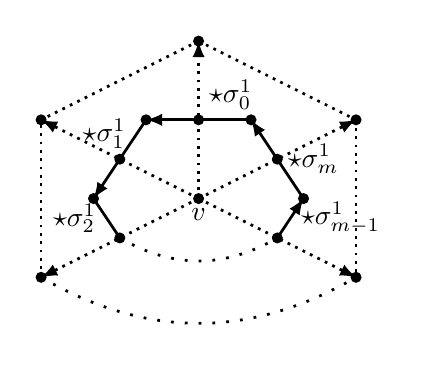
\begin{tikzpicture}[>=latex]
  % Coords
  \coordinate (V0) at (2,0);
  \coordinate (V1) at (2,2);
  \coordinate (V2) at (0,1);
  \coordinate (V3) at (4,1);
  \coordinate (V4) at (4,-1);
  \coordinate (V5) at (0,-1);
  % Arrows\tilde{\sigma}
  \draw[line width=1pt, ->, style=dotted]
    (V0) -- (V1);
  \draw[line width=1pt, style=dotted]
    (V1) --  (V2);
  \draw[line width=1pt, ->, style=dotted]
    (V0) -- (V2);
  \draw[line width=1pt, style=dotted]
    (V1) --  (V3);
  \draw[line width=1pt, ->, style=dotted]
    (V0) -- (V3);
   \draw[line width=1pt, ->, style=dotted]
    (V0) -- (V4);
  \draw[line width=1pt, ->, style=dotted]
    (V0) -- (V5);
  \draw[line width=1pt, style=dotted]
    (V5) --  (V2);
  \draw[line width=1pt, style=dotted]
    (V3) --  (V4);
  % Points
  \fill (V0) node[below] {\(v\)} circle (2pt);
  \fill (V1) circle (2pt);
  \fill (V2) circle (2pt);
  \fill (V3) circle (2pt);
  \fill (V4) circle (2pt);
  \fill (V5) circle (2pt);
  \draw[line width=1pt, style=loosely dotted]
     (V5) to[bend right] (V4);
  %circumcenter
  \coordinate (CC1) at (1.333,1);
  \coordinate (CC0) at (2.666,1);
  \coordinate (CC2) at (0.666,0);
  \coordinate (CCm) at (3.333,0);
  \coordinate (CCC0) at (2,1);
  \coordinate (CCC1) at (1,0.5);
  \coordinate (CCC2) at (3,0.5);
  \coordinate (CCC3) at (1,-0.5);
  \coordinate (CCC4) at (3,-0.5);
  \fill (CC0) circle (2pt);
  \fill (CC1) circle (2pt);
  \fill (CC2) circle (2pt);
  \fill (CCm) circle (2pt);
  \fill (CCC0) circle (2pt);
  \fill (CCC1) circle (2pt);
  \fill (CCC2) circle (2pt);
  \fill (CCC3) circle (2pt);
  \fill (CCC4) circle (2pt);
  \draw[line width=1pt, ->] (CC0) -- node[above right] {\(\star\sigma_0^1\)} (CC1);
  \draw[line width=1pt, ->] (CC1) -- node[above left] {\(\star\sigma_1^1\hspace{-6pt}\)}(CC2);
  \draw[line width=1pt, ->] (CCm) -- node[right] {\(\star\sigma_m^1\)} (CC0);
  \draw[line width=1pt,] (CC2) -- node[left] {\(\star\sigma_2^1\)} (CCC3);
  \draw[line width=1pt,->] (CCC4) -- node[right] {\(\star\sigma_{m-1}^1\)} (CCm);
  \draw[line width=1pt, style=loosely dotted]
     (CCC3) to[bend right] (CCC4);

	
\useasboundingbox ([shift={(1mm,1mm)}]current bounding box.north east) rectangle ([shift={(-1mm,-1mm)}]current bounding box.south west);
\end{tikzpicture}


    \end{minipage}
    \hfill
    \begin{minipage}[b]{0.6\textwidth}
    \begin{align}
    \begin{aligned}
      \left\langle -\delta\alpha,v \right\rangle
          &= \left\langle *\exd * \alpha , v \right\rangle \\
          &= \frac{1}{\left| \star v \right|} \left\langle \exd * \alpha , \star v \right\rangle \\
          &= \frac{1}{\left| \star v \right|} \sum_{i=0}^{m} \left\langle *\alpha , \star\sigma^{1}_{i} \right\rangle \\
          &= \frac{1}{\left| \star v \right|} \sum_{i=0}^{m} \frac{\left| \star\sigma^{1}_{i} \right|}{\left|\sigma^{1}_{i} \right|}
                                                              \left\langle \alpha , \sigma^{1}_{i} \right\rangle
    \end{aligned}
    \end{align}
    \end{minipage}
  \end{beispiel}

  \begin{bemerkung}[zur Implementierung]
    Prinzipiell können alle hier vorgestellten Operatoren als Matrizen implementiert werden, da sie linear sind, vergleiche \cite{siggraphKap7} und \cite{siggraphKap8}.
    Das wollen wir hier nicht machen, da hier das Interface und die Methodik von AMDiS genutzt werden soll.
    Das heißt FEM-typisch werden die Operatoren auf den Dreieckelementen aufgestellt und bilden somit Elementmatrizen, die dann erst zu einer Systemmatrix aufassembliert werden.
    Da AMDiS von Haus aus eine geeignete Speicherstruktur für skalarwertige oder vektorisierte skalarwertige Probleme mitbringt, müssen intern nur die FEM-Operatoren durch geeignete
    DEC-Operatoren ausgetauscht werden.
    Die Problemformulierung, das aufaddieren der Elementmatrizen sowie das Lösen des Gleichungssystem bleibt somit im Ursprünglichen Zustand erhalten.
    Es ist somit sogar möglich Differentialgleichungssysteme mit DEC und FEM in einer einzelnen Problemformulierung gemischt zulösen.
  \end{bemerkung}

  \begin{fazit}
    Auf einer 2-Mannigfalltigkeit lässt sich noch ein weiterer aus der klassischen Vektoranalysis bekannter Ableitungsoperator mit Hilfe der Koableitung darstellen.
    Für \( f\in C^{\infty(M)} \) definiert sich die Rotation über
    \begin{align}
      \left( *\delta\left( *f \right) \right)^{\sharp} = -\left( *\exd f \right)^{\sharp} =: -\text{Rot} f \formpunkt
    \end{align}
    Damit können wir analog zu \eqref{diag2DimAusAbleitung} zusammenfassend den Kettenkomplex mit den zugehörigen Skalar-/Vektorfeldübersetzungsisomorphismen aufstellen:
    \begin{align}
      \begin{xy} \xymatrix{
        \Omega^{0}(M) \ar[d]_{\text{id}} & \Omega^{1}(M) \ar[l]^{\delta} \ar@<2pt>[d]^{\sharp} & \Omega^{2}(M) \ar[l]^{\delta}\\
        C^{\infty}(M) & \mathcal{V}^{\infty}(M) \ar[l]_{\text{Div}} \ar@<2pt>[u]^{\flat} & C^{\infty}(M) \ar[l]_{\text{-Rot}} \ar[u]_{*} }
      \end{xy}
    \end{align}
    Nach dem Baukastenprinzip ließen sich somit alle linearen Differentialgleichungen endlicher Ordnung diskretisieren.
    Um auch nichtlineare Terme wie die Kontraktion (inneres Produkt) \( i_{\vec{v}}\alpha\in\Omega^{p-1}(M) \) 
    oder die Lie-Ableitung \( \mathcal{L}_{\vec{v}}\alpha\in\Omega^{p}(M) \) für \( \vec{v}\in\mathcal{V}^{\infty} \) und \( \alpha\in\Omega^{p}(M) \) darzustellen
    benötigen wir noch das diskrete Dachprodukt \( \wedge \).
    In \cite{desbrun} werden zwei diskretes Dachprodukt auf \( \Omega_{d}^{p}(K)\times\Omega_{d}^{q}(K) \) bzw. \( \Omega_{d}^{p}(\star K)\times\Omega_{d}^{q}(\star K) \)
    für \( p+q\le n \) vorgestellt, welche, wie auch das Dachprodukt für Differentialformen, antikommutativ sind und die Leibnitzregel (Produktregel) bzgl. der äußeren Ableitung erfüllen.
    Allerdings sind sie im Allgemeinen nicht assoziativ im Gegensatz zum stetigen Vorbild.
    In \cite{diskreteLie} gibt es einen anschaulichen Ansatz zur Diskretisierung der Kontraktion.
    Damit könnten wir auch ohne Dachprodukt über Cartans "`magische"' Formel
    \begin{align}
      \mathcal{L}_{\vec{v}}\alpha = i_{\vec{v}}\exd\alpha + \exd i_{\vec{v}}\alpha 
    \end{align}
    als algebraische Bedingung eine diskrete Lie-Ableitung erhalten.
    Somit könnte zum Beispiel auch der Jacobian
    \begin{align}
      \mathcal{J}(\psi,\Delta\psi) = *\exd\mathcal{L}_{\vec{u}}\vecflat{u} 
    \end{align}
    mit dem Strömungsfeld \( u = \text{Rot}\psi\in\mathcal{V}^{\infty}(M) \) und der Stromfunktion \( \psi\in C^{\infty}(M) \),
    wie er in der Wirbelgleichung in \cite{nitschke} vorkommt, numerisch mit Hilfe des DECs als skalarwertiges Problem behandelt werden.
    Auch eine direkte Diskretisierung des Konvektionstermes \( \mathcal{L}_{\vec{u}}\vecflat{u} \) in den Navier-Stokes-Gleichungen (vgl. \cite{Marsden}, Kap.8) wäre denkbar.
    Das Problem an dem resultierendem (Tangential-)Vektorproblem ist, dass wir noch keine diskreten Übersetzungisomorphismen \( \sharp \) und \( \flat \) haben.
    Diese müssten in zukünftigen Arbeiten noch sinnvoll entwickelt werden.
    Erste Ansätze dazu finden sich zum Beispiel in \cite{hirani}.
    Vorher müssten allerdings noch fundamentale implementiertechnische Fragen gestellt werden.
    Wollen wir mit \( 1 \)-Formen oder mit Vektorfeldern speicherintern arbeiten und bei Bedarf die Indizes rauf bzw. herunter ziehen?
    Und wie wollen wir speichern?
    Bei \( 1 \)-Formen ist es klar, im diskreten definieren sie sich über die Werte auf den Kanten, das heißt ein Freiheitsgrad auf jeder Kante.
    Bei Vektorfeldern wird es da schon schwieriger. Am sichersten ist es diese auf den Dreieckelementen zu speichern (effektiv 2 Freiheitsgrade pro Element), da es dort einen eindeutigen
    Tangentialraum auf dem Polytop gibt. 
    Tangentialvektoren auf den Ecken zuspeichern, wie es im flachen Fall üblich ist, wird zu Problemen führen, da auf den Ecken kein eindeutiger Tangentialraum definiert ist.
    Eine Mittelung der umliegenden Tangentialräume der anliegenden Dreiecke (oder auch Kanten) scheint doch recht wilkürlich zu sein und könnte zu einem nicht lösbaren Gleichungssystem
    führen. Es müssen drei Freigheitsgrade für die Ecken angesetzt werden für ein eigentlich zweidimensionales Problem, was zu einem überbestimmten System führen könnte.
    Auf jeden Fall würde es die (dünnbesetzte) Systemmatrix unnötig "`aufblähen"'.

    Wir haben gezeigt, dass für ein immer feiner werdendes wohlzentriertes Primärgitter der diskrete Hodge-Stern-Operator gegen den Hodge-Stern-Operator für Differentialformen auf dem
    zugehörigen Polytop konvergiert.
    Offen für zukünftige Arbeiten bleibt die Frage wie gut denn überhaupt eine Differentialform auf einem Polytop eine Differentialform auf einer glatten Mannigfaltigkeit zu approximieren vermag
    und in welchem Sinne.
    Auf dem Primärgitter ließe sich diese Frage noch am einfachsten beantworten, da dort auf einem Simplex, nach dem Mittelwertsatz der Differentialrechnung, der Tangentialraum an
    wenigstem einem Punkt auf dem zugehörigen abstrakten Simplex übereinstimmt, d.h. dort hätten wir zumindestens schonmal einen gemeinsamen Vektorraum zum vergleichen.
    Für ein Simplex auf dem Dualgitter, wie wir es für den Hodge-Stern-Operator bräuchten, scheint die Situation schwieriger, da hier im allgemeinen die Ecken nicht auf der Mannigfaltigkeit
    liegen und es somit noch unklar ist ob sich überhaupt ein gemeinsamer Tangentialraum finden lässt.
  \end{fazit}




\section{Laplace-Operator}
  
  \begin{ziel}
    Wenn es um Numerik partieller Differentialgleichungen geht, dann liegt der Schwerpunkt oftmals auf der Diskretisierung des Laplace-Operators bzw. Gleichungen der Form
    \begin{align}
      \label{eqAllgemeineLaplaceGleichung}
      \Delta u &= F(u)
    \end{align}
    mit zum Beispiel linearem \( F \) und Skalarfeld oder Vektorfeld \( u \).
    Auch Zeitabhängige Probleme sind denkbar, die durch eine Methode der Wahl in der Zeit diskretisiert werden 
    und somit in jedem Zeitschritt auch in die Kategorie \eqref{eqAllgemeineLaplaceGleichung} passen.

    Wir werden hier den Laplace-Operator für skalare Größen diskretisieren um einen diskreten Laplace-Beltrami-Operator zuerhalten und diesen in der Poisson-Gleichung als Minimalbeispiel
    auch testen. Desweiteren kann der Laplace-Operator auch zur Bestimmung der mittleren Krümmung benutzt werden wie wir in \ref{subsecKruemmungsvektor} noch sehen werden.
    Da hier Oberflächen ohne Rand betrachtet werden, wird auch keine Behandlung von Randbedingungen
    benötigt.
  \end{ziel}

  \subsection{Laplace-Beltrami-Operator}
    Wer sich mit Differentialoperatoren auf Mannigfaltigkeiten beschäftigt wird bald feststellen, dass es
    einen ganzen Zoo von Laplace-Operatoren gibt.
    Da es hier um das äußere Kalkül geht, werden wir hier und im Folgenden den Laplace-de-Rham-Operator,
    auch Hodge-Laplace-Operator genannt, benutzen, denn er definiert sich auf \( p \)-Formen und bildet
    auch auf diese wieder ab.
    \begin{align}
      \Delta_{dR} := \exd\delta + \delta\exd: \Omega^{p}(M) \rightarrow \Omega^{p}(M)
    \end{align}
    Speziell für \( 0 \)-Formen ergibt sich \( \Delta_{dR} = \delta\exd \), da die Koableitung \( 0
    \)-Formen auf \( 0 \) abbildet.
    Das ist gerade der negative Laplace-Beltrami-Operator
    \begin{align}
      \label{eqBeltramiAussenDef}
      \Delta_{B}f := \text{Div}\nabla f = -\delta\exd f = -\Delta_{dR} f
    \end{align}
    für eine Funktion \( f\in C^{\infty}(M) \).
    Wegen der unterschiedlichen Vorzeichen des Laplace-Beltrami-Operators und des Laplace-de-Rham-Operators
    für \( 0 \)-Formen ist Obacht geboten, da dies Grund zur Verwirrung sein könnte.
    Mit einer Riemann-Metrik \( g \) ergibt sich somit
    \begin{align}
      \Delta_{B} f &= \frac{1}{\sqrt{\left| \det g \right|}} \sum_{i,j=1}^{n} \frac{\partial}{\partial x^{j}} \left( g^{ij}\sqrt{\left| \det g \right|} \frac{\partial f}{\partial x^{i}}
      \right) \formpunkt
    \end{align}
    Für eine zweidimensionale Mannigfaltigkeit mit orthogonalen Koordinaten und Metrik \( g=\diag{g_{1},g_{2}} \) lässt sich die Formel vereinfachen zu
    \begin{align}
      \Delta_{B} f &=\sqrt{g^{1}g^{2}} \left(  \frac{\partial}{\partial x^{1}} \left( \sqrt{g^{1}g_{2}} \frac{\partial f}{\partial x^{1}} \right) 
                                             + \frac{\partial}{\partial x^{2}} \left( \sqrt{g_{1}g^{2}} \frac{\partial f}{\partial x^{2}} \right) \right) \formpunkt
    \end{align}
    Der diskrete Laplace-Beltrami-Operator soll der durch \eqref{eqBeltramiAussenDef} DEC-diskretisierte Operator sein.
    In Beispiel \ref{bspDivergenz} wurde die Divergenz an einer Ecke \( v\in K \) schon beschrieben, ebenso die Ableitung an einer Kante in \eqref{eqAbleitungKante}.
    Damit ergibt sich zusammenfassend \\
    \begin{align}
    \begin{aligned}
      \left\langle \Delta_{B} f, v \right\rangle 
          &= \frac{1}{\left| \star v \right|} \sum_{\sigma^{1}\succ v} \frac{\left| \star\sigma^{1} \right|}{\left| \sigma^{1} \right|}
                       \left\langle \exd f , \sigma^{1} \right\rangle \\
          &= \frac{1}{\left| \star v \right|} \sum_{\sigma^{1}=\left[ v,v_{i} \right]} \frac{\left| \star\sigma^{1} \right|}{\left| \sigma^{1} \right|}
                       \left( f(v_{i}) - f(v) \right) \formpunkt
    \end{aligned}
    \end{align}
    

  \subsection{Beispiel: Poisson-Gleichung}

\section{Approximation der Krümmung}
  \subsection{Beispiel: Krümmung Teil 1: Gauß-Bonnet-Operator}
  \subsection{Beispiel: Krümmung Teil 2: Weingarten-Abbildung}
  \subsection{Beispiel: Krümmung Teil 3: Krümmungsvektor}
  \label{subsecKruemmungsvektor}


